
\BookRecordIndex{T0143}格罗莫夫--威滕不变量可以解释为对\BookRecordIndex{T0358}辛流形中孤立的 \BookRecordIndex{T0003}$J$-全纯曲线进行计数。这里所谓
\emph{孤立曲线}，是指它属于一个零维\BookRecordIndex{T0246}模空间。用 Kontsevich--Manin \srcite{216} 的
记号，几何图景如下。

设 $(M,\omega)$ 是紧\BookRecordIndex{T0358}辛流形，固定同调类 $A\in H_2(M;\mathbb Z)$ 以及两个非负整数
$k$ 和 $g$。给定被 $\omega$ \BookRecordIndex{T0372}驯服的\BookRecordIndex{T0088}殆复结构 $J\in\mathcal J_\tau(M,\omega)$，我们
关心紧化\BookRecordIndex{T0246}模空间 $\overline{\mathcal M}_{g,k}(A;J)$：它由 $M$ 中表示同调类 $A$、带
$k$ 个\BookRecordIndex{T0066}标记点的亏格 $g$ 的 \BookRecordIndex{T0003}$J$-全纯曲线组成。在这一一般框架中，不固定某个特定黎曼
曲面 $\Sigma$ 上的复结构，而是考虑所有亏格 $g$ 的 \BookRecordIndex{T0003}$J$-全纯曲线；紧化应在
格罗莫夫--Kontsevich 意义下理解为带 $k$ 个\BookRecordIndex{T0066}标记点的亏格 $g$ \BookRecordIndex{T0340}稳定映射（$g=0$ 时见
第~\ref{ch:stable-maps} 章）。这个\BookRecordIndex{T0246}模空间带有到 $M^k$ 的自然\BookRecordIndex{T0283}求值映射，以及到带 $k$
个\BookRecordIndex{T0066}标记点的亏格 $g$ \BookRecordIndex{T0339}稳定曲线之 Deligne--Mumford 空间
$\overline{\mathcal M}_{g,k}$ 的自然投影，即\BookRecordIndex{T0377}遗忘映射。后一个空间具有紧轨形结构；在
亏格零时，它还是光滑紧流形。（$g=0$ 的介绍见附录 D；任意 $g$ 的介绍见
\srcite{337}。）考虑交换图
\[
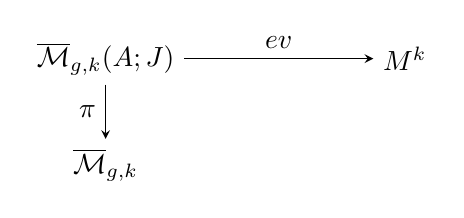
\begin{tikzpicture}[baseline=(current bounding box.center),>=stealth]
  \node (mod) at (0,0) {$\overline{\mathcal M}_{g,k}(A;J)$};
  \node (mk) at (3.8,0) {$M^k$};
  \node (dm) at (0,-1.35) {$\overline{\mathcal M}_{g,k}$};
  \draw[->] (mod) -- node[above] {$\operatorname{ev}$} (mk);
  \draw[->] (mod) -- node[left] {$\pi$} (dm);
\end{tikzpicture}
\]
暂且假装这三个空间都是光滑紧流形。此时，\BookRecordIndex{T0143}格罗莫夫--威滕不变量可以解释为群同态
\[
  \operatorname{GW}^{M}_{g,k,A}:
  H^*(M;\mathbb Q)^{\otimes k}\otimes
  H_*\bigl(\overline{\mathcal M}_{g,k};\mathbb Q\bigr)
  \longrightarrow\mathbb Q,
\]
其定义为
\[
  \operatorname{GW}^{M}_{g,k,A}(a_1,\ldots,a_k;\beta)
  :=\int_{\overline{\mathcal M}_{g,k}(A;J)}
  \operatorname{ev}_1^*a_1\smile\cdots\smile
  \operatorname{ev}_k^*a_k\smile\pi^*\operatorname{PD}(\beta).
\]
从几何上看，可以把这个不变量理解为对如下曲线计数：带 $k$ 个\BookRecordIndex{T0066}标记点的亏格 $g$
\BookRecordIndex{T0003}$J$-全纯曲线，在第 $i$ 个\BookRecordIndex{T0066}标记点处通过与 $a_i$ 庞加莱对偶的循环 $X_i\subset M$，并且
曲线在投影 $\pi$ 下的像被限制在表示类 $\beta$ 的循环
$Y\subset\overline{\mathcal M}_{g,k}$ 中。只要各类 $a_i$ 与 $\beta$ 满足维数条件
\[
  \sum_{i=1}^k\deg(a_i)
  =n(2-2g)+2c_1(A)+\deg(\beta),
\]
原则上这一构造应当给出一个零维约化\BookRecordIndex{T0246}模空间。

所得不变量取有理数值；\BookRecordIndex{T0246}模空间 $\overline{\mathcal M}_{g,k}$ 和
$\overline{\mathcal M}_{g,k}(A;J)$ 都有轨形奇点。前者是因为黎曼曲面可能有非平凡
自同构，后者则是因为\BookRecordIndex{T0113}多重覆盖曲线处可能有非平凡\BookRecordIndex{T0342}稳定子群。

要在完全一般的情形下精确定义这些不变量，需要在紧化\BookRecordIndex{T0246}模空间
$\overline{\mathcal M}_{g,k}(A;J)$ 上构造有理基本循环。这是一个远超本书范围的漫长故事
（参见第~6 章最末的讨论）。本章只解释这幅图景中的一小部分。第一，我们只考虑亏格零；
第二，只考虑\BookRecordIndex{T0058}半正\BookRecordIndex{T0358}辛流形 $(M,\omega)$；第三，只考虑\BookRecordIndex{T0246}模空间
$\overline{\mathcal M}_{0,k}$ 中特殊的同调类 $\beta$，也就是固定指标集
$\{1,\ldots,k\}$ 的某个子集 $I$ 所对应的\BookRecordIndex{T0066}标记点而得到的那些类。最后一个限制并非真正
必要，而且很容易去掉，因为 $\overline{\mathcal M}_{0,k}$ 的同调已经得到充分理解。
不过，另外两个限制（亏格零和\BookRecordIndex{T0058}半正性）在本书发展的分析框架中是本质的。需要强调的是，
\BookRecordIndex{T0058}半正情形下的亏格零不变量在整系数（上）同调类上取整数值。

\BookRecordIndex{T0058}半正流形的亏格零不变量最早由 Ruan \srcite{342,340} 引入辛几何。
\personlater{geluomofu}{格罗莫夫}{Gromov}在 \srcite{160} 中、McDuff 在
\srcite{259} 中曾用其特殊情形研究\BookRecordIndex{T0358}辛流形的结构。\BookRecordIndex{T0150}固定标记点的不变量出现在 sigma 模型
的语境中，并由 Witten \srcite{421} 研究。设
$\beta_{k,I}\in H_{2(k-\#I)}(\overline{\mathcal M}_{0,k};\mathbb Z)$ 的庞加莱对偶，是
最高维群 $H^{2\#I-6}(\overline{\mathcal M}_{0,I};\mathbb Z)$ 的生成元在投影
\[
  \pi_{k,I}:\overline{\mathcal M}_{0,k}\longrightarrow
  \overline{\mathcal M}_{0,I}
\]
下的拉回；与这些同调类 $\beta_{k,I}$ 相联系的亏格零不变量，对应于 Ruan--Tian
\srcite{345} 所谓的\emph{\BookRecordIndex{T0172}混合不变量}，其中只固定指标集 $I$ 所对应的\BookRecordIndex{T0066}标记点。
Kontsevich 和 Manin 在 \srcite{216} 中把\BookRecordIndex{T0143}格罗莫夫--威滕不变量表成群同态
\[
  \operatorname{GW}^{M}_{g,k,A}:
  H^*(M;\mathbb Q)^{\otimes k}
  \longrightarrow H^*(\overline{\mathcal M}_{g,k};\mathbb Q).
\]
按他们的术语，\BookRecordIndex{T0066}标记点可变（$\beta=[\overline{\mathcal M}_{0,k}]$）的不变量是余维零类，
\BookRecordIndex{T0066}标记点固定（$\beta=[\mathrm{pt}]$）的不变量是最高余维类，\BookRecordIndex{T0172}混合不变量则是中间情形
（$\beta_{k,I}$ 对应余维 $2\#I-6$）
\sourcefootnote{原书把 $\overline{\mathcal M}_{0,I}$ 的最高维上同调群印作
$H^{\#I-3}$，并把 $\beta_{k,I}$ 的余维印作 $2\#I$；但
$\dim_{\mathbb R}\overline{\mathcal M}_{0,I}=2\#I-6$，且
$\beta_{k,I}\in H_{2(k-\#I)}(\overline{\mathcal M}_{0,k})$，故两处次数都唯一应为
$2\#I-6$。}。下文省略自变量 $\beta$ 和亏格指标，并把与
$\beta_{k,I}$ 相联系的亏格零不变量记作 $\operatorname{GW}^{M,I}_{A,k}$。当
$\#I=3$ 时，简写为
$\operatorname{GW}^{M}_{A,k}:=\operatorname{GW}^{M,I}_{A,k}$。若从上下文可知流形 $M$，
则省略上标 $M$。

本章首先仔细定义计数不变量 $\operatorname{GW}$，并给出最初的一批例子。为方便读者，
其中也讨论前几章的一些相关结果。第~\ref{sec:7-2} 节发展主构造的若干变体；例如，我们
为以固定树为模型的曲线以及固定某个\BookRecordIndex{T0066}标记点子集的曲线定义不变量。我们还讨论\BookRecordIndex{T0399}障碍丛，
它使我们能够用非正则但足够良好的\BookRecordIndex{T0088}殆复结构来计算不变量。第~\ref{sec:7-3} 节引入与
\BookRecordIndex{T0335}伪全纯图像相联系的不变量 $\operatorname{GW}^I$，并把它们与 $\operatorname{GW}$ 联系
起来。第~\ref{sec:7-4} 节用射影空间中的曲线为例说明这些思想。最后一节叙述
\BookRecordIndex{T0143}格罗莫夫--威滕不变量的 Kontsevich--Manin 公理，并用 $\operatorname{GW}^I$ 解释这些
公理。为展示其威力，我们还会给出 Kontsevich 对 $\mathbb{CP}^2$ 中通过 $3d-1$ 个一般
点的 $d$ 次\BookRecordIndex{T0386}有理曲线数 $N_d$ 的计算。全章都限于亏格零；第~8 章会讨论一些高亏格例子，
见例~\ref{ex:8-6-12}。

\section{计数伪全纯球面}\label{sec:7-1}
\zhindex{jishuweiquanchunqiumian}{计数伪全纯球面}

本节定义\BookRecordIndex{T0143}格罗莫夫--威滕不变量 $\operatorname{GW}_{A,k}$，并在一些简单情形下计算它们。
在给出正式定义之前，我们先说明庞加莱对偶与\BookRecordIndex{T0337}伪循环的若干事项。

与第~\ref{sec:6-5} 节一样，以下用记号
\[
  H^*(M):=H^*(M;\mathbb Z)/\operatorname{Tor}
\]
表示 $H^*(M;\mathbb Z)$ 的自由部分，同调群也采用类似记号。依定义，奇异上同调类
$a\in H^k(M)$ 由它在 $H_*(M)$ 中各同调类上的取值唯一确定，并可等同于相应的群同态
$H_*(M)\to\mathbb Z$。若一个 $(2n-k)$ 维\BookRecordIndex{T0337}伪循环 $f:U\to M$ 对每个闭定向 $k$ 维
子流形 $X\subset M$ 都满足
\[
  \int_X a=f\cdot X,
\]
就称 $f$ 与 $a$（庞加莱）对偶。于是，若 $f:U\to M$ 与 $a$ 对偶，而
$g:V\to M$ 与 $b$ 对偶，则
\[
  \int_M a\wedge b=f\cdot g
\]
（见引理~\ref{lem:6-5-7}）。用第~\ref{sec:6-5} 节的术语，与上同调类 $a$ 对偶的
\BookRecordIndex{T0337}伪循环，是同调类 $\operatorname{PD}(a)$ 的\BookRecordIndex{T0292}弱代表元。

现在设 $(M,\omega)$ 是闭\BookRecordIndex{T0058}半正辛 $2n$ 维流形，$A\in H_2(M;\mathbb Z)$ 是满足
式~\eqref{eq:6-6-1} 的球面同调类，且 $k$ 是非负整数。定理~\ref{thm:6-6-1} 断言，对
每个 $J\in\mathcal J_{\mathrm{reg}}(M,\omega)$（见定义~\ref{def:6-2-1}），\BookRecordIndex{T0283}求值映射
\[
  \operatorname{ev}_J:\mathcal M^*_{0,k}(A;J)\longrightarrow M^k
\]
都是维数
\[
  \mu(A,k):=2n+2c_1(A)+2k-6
\]
的\BookRecordIndex{T0337}伪循环。

\begin{theorem}\label{thm:7-1-1}
设 $(M,\omega)$ 是闭\BookRecordIndex{T0058}半正辛 $2n$ 维流形，$k$ 是非负整数，而
$A\in H_2(M;\mathbb Z)$ 是球面同调类，并且不是任何满足 $c_1(B)=0$ 的球面同调类
$B$ 的非平凡整数倍。则由
\begin{equation}\label{eq:7-1-1}
  \operatorname{GW}^{M}_{A,k}(a_1,\ldots,a_k):=f\cdot\operatorname{ev}_J
\end{equation}
定义的群同态
\[
  \operatorname{GW}^{M}_{A,k}:H^*(M)^{\otimes k}\longrightarrow\mathbb Z
\]
与\BookRecordIndex{T0088}殆复结构 $J$ 以及定义它所用的\BookRecordIndex{T0337}伪循环 $f$ 无关。这里
$J\in\mathcal J_{\mathrm{reg}}(M,\omega)$，而 $f:U\to M^k$ 是与
$\pi_1^*a_1\smile\cdots\smile\pi_k^*a_k$ 庞加莱对偶的\BookRecordIndex{T0337}伪循环，
$\pi_i:M^k\to M$ 表示到第 $i$ 个因子的投影。
\end{theorem}

\begin{proof}
由定理~\ref{thm:6-6-1}，$\operatorname{ev}_J$ 的配边类与 $J$ 无关。因此，由
引理~\ref{lem:6-5-5}，交数 $f\cdot\operatorname{ev}_J$ 与 $J$ 无关。再由
引理~\ref{lem:6-5-7}，它只依赖于\BookRecordIndex{T0337}伪循环 $f$ 所表示的同调类。这就证明了定理。
\end{proof}

上述群同态
$\operatorname{GW}^{M}_{A,k}:H^*(M)^{\otimes k}\to\mathbb Z$
称为 $(M,\omega)$ 在同调类 $A$ 中的\emph{$k$ 点亏格零\BookRecordIndex{T0143}格罗莫夫--威滕不变量}。

\begin{exercise}\label{ex:7-1-2}
证明：$\operatorname{GW}^{M}_{A,k}(a_1,\ldots,a_k)$ 也可定义为
$\operatorname{ev}$ 与乘积循环 $f_1\times\cdots\times f_k$ 的交数，其中
$f_j:U_j\to M$ 分别是与上同调类 $a_j$ 对偶的\BookRecordIndex{T0337}伪循环。换言之，可以在乘积循环这一类
之内达到横截。

\emph{提示：}把引理~\ref{lem:6-5-5}(i) 略作修改，用于 $f$ 是乘积循环而 $\phi$
是乘积微分同胚的情形。
\end{exercise}

回忆第~6 章，当 $A\ne0$ 时，\BookRecordIndex{T0246}模空间 $\mathcal M^*_{0,k}(A;J)$ 是元组
$(u,z_1,\ldots,z_k)$ 的等价类之集，其中 $u:S^2\to M$ 是表示类 $A$ 的单纯
$J$-全纯球面，而 $z_i$ 是 $S^2$ 上两两不同的点。等价关系由\BookRecordIndex{T0413}重参数化群
$G=\operatorname{PSL}(2,\mathbb C)$ 的自然作用给出。由定理~\ref{thm:3-1-6}，对每个
$J\in\mathcal J_{\mathrm{reg}}(A)$，这个空间都是维数为 $\mu(A,k)$ 的光滑定向流形。
定理~\ref{thm:6-6-1} 更强的断言，即它对每个
$J\in\mathcal J_{\mathrm{reg}}(M,\omega)$ 都是\BookRecordIndex{T0337}伪循环，意味着紧化中出现的所有\BookRecordIndex{T0072}层维数
至多为 $\mu(A,k)-2$。现在设每个类 $a_i\in H^*(M)$ 都与一般位置的定向子流形
$X_i\subset M$ 对偶。此时，\BookRecordIndex{T0143}格罗莫夫--威滕不变量
$\operatorname{GW}^{M}_{A,k}(a_1,\ldots,a_k)$ 就是类 $A$ 中通过各子流形 $X_i$ 的
$J$-全纯球面的带适当符号计数：
\[
  \operatorname{GW}^{M}_{A,k}(a_1,\ldots,a_k)
  =\#\Bigl\{[u,z_1,\ldots,z_k]\in\mathcal M^*_{0,k}(A;J)
  \ \Big|\ u(z_i)\in X_i\Bigr\}.
\]
只要各类 $a_i$ 的次数之和等于\BookRecordIndex{T0246}模空间维数，这个公式作为模 $2$ 不变量便是严格成立的：
\begin{equation}\label{eq:7-1-2}
  \sum_{i=1}^k\deg(a_i)=\mu(A,k)=2n+2c_1(A)+2k-6.
\end{equation}
在其余所有情形，不变量依定义为零。注意，一般位置假设不仅意味着\BookRecordIndex{T0283}求值映射横截于
$X_1\times\cdots\times X_k$，还意味着这个乘积不与紧化中各低维\BookRecordIndex{T0072}层所对应\BookRecordIndex{T0283}求值映射的像
相交。

\begin{example}\label{ex:7-1-3}
情形 $A=0$ 需要单独讨论。由于每个常值分支必须带至少三个\BookRecordIndex{T0320}特殊点，
$\mathcal M^*_{0,k}(0;J)$ 在 $k<3$ 时为空。当 $k\ge3$ 时，它由元组
$(x,z_1,\ldots,z_k)$ 组成，其中 $x\in M$（把它看作常值 $J$-全纯球面
$u(z)\equiv x$），而 $z_i$ 是 $S^2$ 上两两不同的点。当 $k>3$ 时，式~\eqref{eq:7-1-2}
说明，与类 $a_i$ 对偶的循环 $X_i$ 的总余维严格大于 $2n$，故它们处于一般位置时没有
交点。因此，$A=0$ 的\BookRecordIndex{T0143}格罗莫夫--威滕不变量在 $k\ne3$ 时为零。若 $k=3$，数
$\operatorname{GW}^{M}_{0,3}(a_1,a_2,a_3)$ 计数各庞加莱对偶的三重交。这说明
\[
  \operatorname{GW}^{M}_{0,3}(a_1,a_2,a_3)
  =\int_M a_1\smile a_2\smile a_3.
\]
\end{example}

\begin{example}\label{ex:7-1-4}
另一个有趣的特殊情形是 $k=0$。若同时有 $A=0$，便没有可计数的对象，我们把不变量
定义为零。不过，当 $A\ne0$ 时，可以把流形 $M^k$ 看成一个点，从而定义\BookRecordIndex{T0348}相容且有趣的
不变量。只要 $J\in\mathcal J_{\mathrm{reg}}(A)$，且\BookRecordIndex{T0246}模空间
$\mathcal M^*_{0,0}(A;J)$ 的维数
$\mu(A,0)=2n+2c_1(A)-6$ 大于零，\BookRecordIndex{T0283}求值映射
\[
  \operatorname{ev}_J:\mathcal M^*_{0,0}(A;J)\longrightarrow\{\mathrm{pt}\}
\]
自动是\BookRecordIndex{T0337}伪循环。然而在这种情形，它的同调类由于维数原因等于零。因此，不变量只有在
\[
  2n+2c_1(A)=6
\]
时才可能非零，此时\BookRecordIndex{T0246}模空间 $\mathcal M^*_{0,0}(A;J)$ 是零维的。若
$J\in\mathcal J_{\mathrm{reg}}(M,\omega)$，紧化中的所有边界\BookRecordIndex{T0072}层都有负虚维数，因而为空。
于是 $\mathcal M^*_{0,0}(A;J)$ 是有限集，而不变量
\[
  \operatorname{GW}(A):=\operatorname{GW}_{A,0}(1)\in\mathbb Z
\]
是 $\mathcal M^*_{0,0}(A;J)$ 中元素的带适当符号计数。当 $M=S^2$ 且 $c_1(A)=2$ 时，
这个数为一。若 $\dim M=4$、$c_1(A)=1$ 且 $A\cdot A=-1$，不变量计数表示类 $A$ 的例外
除子数目（见下文例~\ref{ex:7-1-15}）。由\BookRecordIndex{T0186}交点正性，这个数只能是零或一。不过，若
$A\cdot A\ge0$，不变量也可能取零、一以外的值（见下文习题~\ref{ex:7-1-17}）。最重要
的情形是 Calabi--Yau 流形（$\dim M=6$ 且 $c_1(A)=0$）。此时，去掉 $A$ 必须是本原类
这一假设至关重要；见注~\ref{rem:7-3-8}。
\end{example}

最后给出两个习题，说明这些不变量的一些基本几何性质；参见第~\ref{sec:7-5} 节列出的
（除子）公理和（基本类）公理。

\begin{exercise}\label{ex:7-1-5}
设 $(M,\omega)$ 是紧辛四维流形，而 $A$ 是满足 $c_1(A)=1$ 的球面同调类。证明：若
$a_k\in H^2(M)$ 且 $k\ge1$，则
\[
  \operatorname{GW}_{A,k}(a_1,\ldots,a_k)
  =\operatorname{GW}_{A,k-1}(a_1,\ldots,a_{k-1})\cdot\int_A a_k.
\]
这里的几何想法是，每条 $A$-曲线与 $\operatorname{PD}(a_k)$ 相交
$\int_Aa_k$ 次；因此无须分别记录这些交点。
\end{exercise}

\begin{exercise}\label{ex:7-1-6}
设 $(M,\omega)$ 是紧\BookRecordIndex{T0058}半正\BookRecordIndex{T0358}辛流形且 $A\ne0$。证明：当 $k\ge1$ 时，
\[
  \operatorname{GW}_{A,k}(a_1,\ldots,a_{k-1},1)=0,
\]
其中 $1:=\operatorname{PD}([M])\in H^0(M)$。这里的想法是，由于最后一个\BookRecordIndex{T0066}标记点不受
约束，相关交点永远不是孤立的，故不变量为零。
\end{exercise}

\paragraph{关于定义的说明。}

\paragraph{\BookRecordIndex{T0058}半正性。}
如果不存在满足
\[
  \omega(A)>0,
  \qquad
  2-n<c_1(A)<0
\]
的球面同调类 $A\in H_2(M;\mathbb Z)$，就称紧\BookRecordIndex{T0358}辛流形 $(M,\omega)$ 是\BookRecordIndex{T0058}半正的。特别地，
每个维数 $2n\le6$ 的\BookRecordIndex{T0358}辛流形都满足这一条件。正如第~\ref{sec:6-4} 节所解释的，这一条件
保证：对通有的 $J$，不存在第一陈数为负的 $J$-全纯球面。要理解其意义，先回忆：若
\BookRecordIndex{T0340}稳定映射的每个非常值分支都是单纯的（即不是多重覆盖），并且任意两个非常值分支的像
都不同，就称它为\BookRecordIndex{T0184}简单稳定映射。其次，只要 $J\in\mathcal J_{\mathrm{reg}}(M,\omega)$，
以带 $k$ 个标号的树 $T$ 为模型的\BookRecordIndex{T0184}简单稳定映射\BookRecordIndex{T0246}模空间
$\mathcal M^*_{0,T}(B;J)$ 就是维数为 $\mu(B,k)-2e(T)$ 的光滑流形
（定理~\ref{thm:6-2-6}）。第三，对类 $A$ 中每个非\BookRecordIndex{T0184}简单稳定映射，都存在某个类 $B$ 中
的底\BookRecordIndex{T0072}层\BookRecordIndex{T0184}简单稳定映射，它与原\BookRecordIndex{T0340}稳定映射有相同的像，并在各\BookRecordIndex{T0066}标记点处取相同的值
（命题~\ref{prop:6-1-2}）。现在，若每个 $J$-全纯球面的陈数都非负，则
$c_1(B)\le c_1(A)$，所以紧化中的所有边界\BookRecordIndex{T0072}层维数都小于 $\mu(A,k)$
\sourcefootnote{原书此处把比较对象印作 $\mu(A,T)$；但紧邻上文给出的 $T$-\BookRecordIndex{T0072}层预期维数
本身就是 $\mu(B,k)-2e(T)$（当 $B=A$ 时即为 $\mu(A,T)$），而且不同边界\BookRecordIndex{T0072}层的树 $T$
并不固定。\BookRecordIndex{T0337}伪循环论证所需、并由 $e(T)>0$ 得到的统一比较对象，是主\BookRecordIndex{T0072}层维数
$\mu(A,k)$。}。这正是证明
$J\in\mathcal J_{\mathrm{reg}}(M,\omega)$ 时\BookRecordIndex{T0283}求值映射为\BookRecordIndex{T0337}伪循环的关键成分
（定理~\ref{thm:6-6-1}）。若只考虑那些使所有相关 $J$-全纯球面都有非负陈数的\BookRecordIndex{T0088}殆复
结构，便可以放宽\BookRecordIndex{T0058}半正性条件（注~\ref{rem:6-6-2}）。

\paragraph{符号的确定。}
计算\BookRecordIndex{T0143}格罗莫夫--威滕不变量的另一个重要环节，是确定正确的符号。若 $J$ 可积，我们在
注~\ref{rem:3-2-6} 中已经看到，\BookRecordIndex{T0246}模空间带有与其定向\BookRecordIndex{T0348}相容的复结构。因此在这种情形，通常
很容易确定交点符号（见下文例~\ref{ex:7-1-15}）。然而，若 $J$ 不可积，这个问题一般
要微妙得多。

\paragraph{识别正则\BookRecordIndex{T0088}殆复结构。}
为了计算不变量，必须能够识别一个给定\BookRecordIndex{T0088}殆复结构 $J$ 何时属于
$\mathcal J_{\mathrm{reg}}(M,\omega)$。这意味着：对所有单纯 $J$-全纯球面，\BookRecordIndex{T0346}线性化算子
$D_u$ 都满射；并且对所有树，\BookRecordIndex{T0065}边求值映射都横截于\BookRecordIndex{T0061}边对角线（见定义~\ref{def:6-2-1}）。
这些条件蕴含所有\BookRecordIndex{T0184}简单稳定映射的\BookRecordIndex{T0246}模空间都有预期维数，因而对任意 $A$ 和 $k$，
$\operatorname{ev}_J:\mathcal M^*_{0,k}(A;J)\to M^k$ 都是\BookRecordIndex{T0337}伪循环。为计算不变量
$\operatorname{GW}_{A,k}$，只须对确实出现在
$\mathcal M^*_{0,k}(A;J)$ 的紧化中的那些树 $T$ 和同调类 $\{B_\alpha\}$ 验证这些条件。
这些类必须对某组正整数 $m_\alpha$ 满足
\[
  \sum_{\alpha\in T}m_\alpha B_\alpha=A.
\]
当 $A$ 不容许任何这种非平凡分解时，情形尤其简单。

\begin{definition}\label{def:7-1-7}
若类 $A$ 不能写成
\[
  A=A_1+\cdots+A_k,
\]
其中 $k\ge2$，且每个 $A_i$ 都有非常值球面 $J$-全纯代表元，就称 $A$ 是
\emph{\BookRecordIndex{T0002}$J$-不可分解的}。
\end{definition}

\begin{lemma}\label{lem:7-1-8}
设 $A\in H_2(M;\mathbb Z)$ 且 $J\in\mathcal J_{\mathrm{reg}}(A)$（即对每个表示类
$A$ 的单纯 $J$-全纯球面 $u$，$D_u$ 都满射）。若 $A$ 是 \BookRecordIndex{T0002}$J$-不可分解的，则对每个整数
$k\ge0$，\BookRecordIndex{T0283}求值映射
\[
  \operatorname{ev}_J:\mathcal M^*_{0,k}(A;J)\longrightarrow M^k
\]
都是\BookRecordIndex{T0337}伪循环，并且可以用 $\operatorname{ev}_J$ 计算 $\operatorname{GW}_{A,k}$。
\end{lemma}

\begin{proof}
由于 $J\in\mathcal J_{\mathrm{reg}}(A)$，对每个表示类 $A$ 的单纯 $J$-全纯球面
$u:S^2\to M$，算子 $D_u$ 都满射。因此，类 $A$ 中不带标记的单纯 $J$-曲线\BookRecordIndex{T0246}模空间
\[
  \mathcal M^*_{0,0}(A;J)=\mathcal M^*(A;J)/G
\]
是预期维数 $2n+2c_1(A)-6$ 的流形
\sourcefootnote{原书此处漏掉了除以\BookRecordIndex{T0413}重参数化群 $G$ 所减少的六个实维数，把
$\mathcal M^*_{0,0}(A;J)$ 的预期维数印作 $2n+2c_1(A)$；由紧邻的商空间定义以及
$\mu(A,0)=2n+2c_1(A)-6$，唯一应补为这里的数值。}。我们断言它是紧的。首先，由于 $A$ 是
\BookRecordIndex{T0002}$J$-不可分解的，每条表示类 $A$ 的 $J$-曲线都是单纯的。其次，由
定理~\ref{thm:5-3-1}，$\mathcal M_{0,0}(A;J)$ 中任意序列都有\BookRecordIndex{T0141}格罗莫夫收敛子列。由于
没有\BookRecordIndex{T0066}标记点，其极限只有一个分支，因而必属于
$\mathcal M_{0,0}(A;J)=\mathcal M^*_{0,0}(A;J)$。（注意，若在所有具有 $J$-全纯
代表元的类中，$A$ 具有最小能量，那么同一结论也可由简单得多的
定理~\ref{thm:4-2-11} 得到。）

当 $k\ge2$ 时，相应空间 $\mathcal M^*_{0,k}(A;J)$ 不会是紧的，因为\BookRecordIndex{T0066}标记点必须始终
互异。不过，位于边界\BookRecordIndex{T0072}层的\BookRecordIndex{T0340}稳定映射由一个表示类 $A$ 的主分支，以及若干用于容纳\BookRecordIndex{T0066}标记点
的\BookRecordIndex{T0382}幽灵分支组成。这些\BookRecordIndex{T0072}层总是正则的，而且维数为 $\mu-2e(T)$（见
习题~\ref{ex:7-1-9}）。因此，紧化中的所有\BookRecordIndex{T0072}层都有预期维数，引理得证。
\end{proof}
\begin{exercise}\label{ex:7-1-9}
设 $A$ 是 \BookRecordIndex{T0002}$J$-不可分解的，且
$J\in\mathcal J_{\mathrm{reg}}(A,\mathbb{CP}^1)$。则类 $A$ 中每个\BookRecordIndex{T0340}稳定映射都包含一个
表示类 $A$ 的主分支，还可能包含若干带有\BookRecordIndex{T0066}标记点的\BookRecordIndex{T0382}幽灵分支。验证：对每棵树 $T$，都有
$J\in\mathcal J_{\mathrm{reg}}(A,T)$。（参见习题~\ref{ex:6-2-5}。）
\end{exercise}

\begin{exercise}\label{ex:7-1-10}
设 $A\in H_2(M;\mathbb Z)$。证明：使 $A$ 为 \BookRecordIndex{T0002}$J$-不可分解类的所有被 $\omega$ \BookRecordIndex{T0372}驯服
\BookRecordIndex{T0088}殆复结构 $J$，在 $\mathcal J_\tau(M,\omega)$ 中构成开集。
\end{exercise}

\begin{remark}\label{rem:7-1-11}
\BookRecordIndex{T0363}辛形式 $\omega$ 的一个\emph{形变}，是从 $\omega_0=\omega$ 出发的\BookRecordIndex{T0363}辛形式光滑单参数族
\[
  [0,1]\longrightarrow\Omega^2(M),
  \qquad t\longmapsto\omega_t.
\]
与同痕的概念不同，这里不要求上同调类保持不变。由于\BookRecordIndex{T0372}驯服条件是开的，被 $\omega$ \BookRecordIndex{T0372}驯服
的\BookRecordIndex{T0088}殆复结构 $J$ 也被所有充分接近 $\omega$ 的\BookRecordIndex{T0363}辛形式\BookRecordIndex{T0372}驯服。因此，在 $\omega$ 的形变
$\omega_t$ 下，\BookRecordIndex{T0143}格罗莫夫--威滕不变量 $\operatorname{GW}^{M}_{A,k}$ 不变，只要
对每个 $t\in[0,1]$，$(M,\omega_t)$ 都是\BookRecordIndex{T0058}半正的。
\footnote{当然，一旦构造出\BookRecordIndex{T0370}虚模循环，这个附加条件便不再必要。因此，现在已知这些不变量
只依赖于 $(M,\omega)$ 的形变类型。}
除非碰巧有 $\dim M\le6$ 或 $c_1$ 在 $\pi_2$ 上消失，否则这个关于 $\omega_t$ 的条件
相当苛刻。在上述两种情形中，$(M,\omega_t)$ 对某一个形式 $\omega_t$ \BookRecordIndex{T0058}半正，当且仅当它
对形变中的所有形式 $\omega_t$ 都\BookRecordIndex{T0058}半正。因此在这些情形，\BookRecordIndex{T0143}格罗莫夫--威滕不变量只依赖于
$(M,\omega)$ 的形变类型。四维时还有更强的结论：Taubes 证明，嵌入曲线（可能有更高
亏格）的 Gromov 不变量与 Seiberg--Witten 不变量相同，因而这些 Gromov 不变量只依赖于
$M$ 的光滑结构。不过六维时并非如此；见第~\ref{ch:applications-symplectic-topology} 章关于 Ruan 例子的讨论。
\end{remark}

\begin{remark}[同调的不变量]\label{rem:7-1-12}
到目前为止，我们用 $M$ 的上同调定义\BookRecordIndex{T0143}格罗莫夫--威滕不变量。然而在某些情形，把它们看成
由同调类决定会更方便。给定 $\alpha_1,\ldots,\alpha_k\in H_*(M)$，定义
\[
  \operatorname{GW}^{M}_{A,k}(\alpha_1,\ldots,\alpha_k)
  :=\operatorname{GW}^{M}_{A,k}
  \bigl(\operatorname{PD}(\alpha_1),\ldots,\operatorname{PD}(\alpha_k)\bigr).
\]
它计数\BookRecordIndex{T0283}求值映射
$\operatorname{ev}:\mathcal M^*_{0,k}(A;J)\to M^k$ 与乘积类
$\alpha_1\times\cdots\times\alpha_k\in H_*(M^k)$ 的交数。
\end{remark}

\paragraph{例子。}

\begin{example}\label{ex:7-1-13}
考虑带乘积\BookRecordIndex{T0363}辛形式的乘积流形
\[
  \widetilde M:=S^2\times M,
\]
并假设 $\widetilde M$ \BookRecordIndex{T0058}半正。例如，当 $\dim M\le4$ 或 $\pi_2(M)=0$ 时便是如此。考虑
球面同调类
\[
  \widetilde A:=[S^2\times\mathrm{pt}]
  \in H_2(S^2\times M;\mathbb Z),
\]
并设 $\widetilde J$ 是一个被 $\widetilde\omega$ \BookRecordIndex{T0372}驯服的乘积\BookRecordIndex{T0088}殆复结构。由
推论~\ref{cor:3-3-5}，$\widetilde J\in\mathcal J_{\mathrm{reg}}(\widetilde A)$，而且类
$\widetilde A$ 是 $\widetilde J$-不\BookRecordIndex{T0213}可分解的。此外，通过 $\widetilde M$ 中每一点恰有一个
$\widetilde J$-全纯 $\widetilde A$-球面。因此由引理~\ref{lem:7-1-8}，\BookRecordIndex{T0283}求值映射
\[
  \operatorname{ev}:\mathcal M_{0,1}(\widetilde A;\widetilde J)
  \longrightarrow\widetilde M
\]
是微分同胚。故
\[
  \operatorname{GW}^{\widetilde M}_{\widetilde A,1}(\widetilde a)
  =\int_{\widetilde M}\widetilde a.
\]
\end{example}

\begin{example}[射影空间中的直线]\label{ex:7-1-14}
$\mathbb{CP}^n$ 中任意两点位于唯一一条直线上。这应当转化成公式
\[
  \operatorname{GW}^{\mathbb{CP}^n}_{L,2}(c^n,c^n)=1,
\]
其中
\[
  L:=[\mathbb{CP}^1]\in H_2(\mathbb{CP}^n;\mathbb Z),
\]
$c$ 是 $H^2(\mathbb{CP}^n;\mathbb Z)$ 的正生成元，而
$c^n=\operatorname{PD}([\mathrm{pt}])\in H^{2n}(\mathbb{CP}^n;\mathbb Z)$。为验证这一点，
先注意 $c_1(L)=n+1$ 且 $k=2$，所以维数条件~\eqref{eq:7-1-2} 在
$\mu(L,2)=4n$ 时成立。此外，标准复结构 $J_0$ 满足引理~\ref{lem:3-3-2} 的假设。事实上，
若 $u:\mathbb{CP}^1\to\mathbb{CP}^n$ 是一条直线，则拉回切丛
$u^*T\mathbb{CP}^n\to\mathbb{CP}^1$ 分裂成全纯线丛的直和，其中一个线丛的陈数为二，
其余线丛的陈数为一。陈数为一的线丛可实现为
$\mathbb{CP}^{k-1}\subset\mathbb{CP}^k$ 的\BookRecordIndex{T0117}法丛，其中 $k=2,\ldots,n$。这说明
$J_0\in\mathcal J_{\mathrm{reg}}(L)$。由于 $L$ 是 $J_0$-不\BookRecordIndex{T0213}可分解类，引理~\ref{lem:7-1-8}
断言我们可以用 $J_0$ 计算 $\operatorname{GW}_{L,2}$。因此，
$\operatorname{GW}_{L,2}(c^n,c^n)$ 恰为通过两点的直线数，故等于一。

另一个初等\BookRecordIndex{T0143}格罗莫夫--威滕不变量是
$\operatorname{GW}^{\mathbb{CP}^3}_{L,3}(c^2,c^2,c^3)$。它计数三维射影空间中通过一点
并与两条一般直线相交的直线。维数条件~\eqref{eq:7-1-2} 成立，所以这个数可能非零。
此外，满足这些关联条件的直线唯一，即分别取过该点与其中一条直线的两个平面，它们的
交线。为了\BookRecordIndex{T0326}推出
\[
  \operatorname{GW}^{\mathbb{CP}^3}_{L,3}(c^2,c^2,c^3)=1,
\]
还需确认\BookRecordIndex{T0283}求值映射
$\operatorname{ev}:\mathcal M(L,J_0)\to(\mathbb{CP}^3)^3$ 横截于类
$[\mathrm{pt}]\times L\times L$ 的一般代表元。这可以直接验证，也可由下文
命题~\ref{prop:7-4-5} 得到。
\end{example}

\begin{example}[例外除子]\label{ex:7-1-15}
用 $\overline{\mathbb{CP}^2}$ 表示取反向定向的复射影平面。注意，它不是复流形。若
$E\in H_2(\overline{\mathbb{CP}^2};\mathbb Z)$ 表示子流形 $\mathbb{CP}^1$（带标准定向）
的同调类，则 $E\cdot E=-1$。

设 $(M,\omega)$ 是复 凯勒 曲面，而 $(\widetilde M,\widetilde J)$ 表示它在点 $x$ 处的
吹起。这意味着，用所有通过 $x$ 的直线之集替代 $x$。这个直线集是
$\mathbb{CP}^1$ 的一个副本，称为例外除子 $\Sigma$。$\Sigma$ 的\BookRecordIndex{T0117}法丛是
$\mathbb{CP}^1$ 上欧拉类为 $-1$ 的\BookRecordIndex{T0414}重言线丛，由此存在微分同胚
\[
  \widetilde M\cong M\#\overline{\mathbb{CP}^2},
\]
把 $\Sigma$ 识别为 $\overline{\mathbb{CP}^2}$ 中的一条复直线。这个构造在辛范畴中也
成立（见第~\ref{sec:9-3} 节）；特别地，复吹起 $(\widetilde M,\widetilde J)$ 是
凯勒 的。更多细节见第~\ref{sec:9-3} 节。

令 $E=[\Sigma]$ 表示例外除子的同调类。于是，\BookRecordIndex{T0246}模空间
$\mathcal M(E;\widetilde J)$ 在重参数化意义下只含一条 $\widetilde J$-全纯曲线，即例外
除子本身。为说明这一点，注意同一类中的任何另一条 $\widetilde J$-全纯曲线都必须以交数
$-1$ 与 $\Sigma$ 相交；但任意两条不同的 $\widetilde J$-全纯曲线交数非负，这是不可能
的。此外，由引理~\ref{lem:3-3-3}，曲线 $\Sigma$ 正则，这与维数公式
\[
  \dim\mathcal M^*(E;\widetilde J)=4+2c_1(E)=6
\]
相符。因此，由引理~\ref{lem:7-1-8} 和习题~\ref{ex:7-1-5}，
\[
  \operatorname{GW}^{M\#\overline{\mathbb{CP}^2}}_{E,1}
  \bigl(\operatorname{PD}(E)\bigr)=E\cdot E=-1.
\]

于是，对 $\widetilde M$ 上每个被 $\widetilde\omega$ \BookRecordIndex{T0372}驯服的 $J$，类 $E$ 都必须有一个
$J$-全纯代表元。这个代表元可能是可约的。例如，若 $M=\mathbb{CP}^2$，则
$M\#\overline{\mathbb{CP}^2}$ 微分同胚于射影化丛
$\mathbb P(\mathcal L_3\oplus\mathbb C)$，其中线丛
$\mathcal L_3\to\mathbb{CP}^1$ 的陈数为三。子丛 $\mathcal L_3$ 给出
$\mathbb P(\mathcal L_3\oplus\mathbb C)$ 的一个自交数为 $-3$ 的截面，并表示类
\[
  2E-L\in H_2(\mathbb{CP}^2\#\overline{\mathbb{CP}^2};\mathbb Z).
\]
因此，对某个适当的\BookRecordIndex{T0088}殆复结构 $J$，类 $E$ 由这个 $(-3)$-球面与投影
$\mathbb P(\mathcal L_3\oplus\mathbb C)\to\mathbb{CP}^1$ 的纤维 $L-E$ 之并表示。不过，
由于 $(2E-L)$-曲线不可能正则，这种情形对通有的 $J$ 不会发生。
\end{example}

\begin{exercise}\label{ex:7-1-16}
\begin{enumerate}[label=(\roman*),leftmargin=3em]
\item 证明：对 $\mathbb{CP}^2$ 中任意五个点，只要其中没有三个共线，就存在一个二次
齐次多项式 $f$，其零点集通过这五点，并且 $f$ 在非零常数倍意义下唯一
\sourcefootnote{原书说存在“唯一的二次齐次多项式 $f$”，但 $f$ 的任意非零常数倍定义
同一零点集；唯一的是 $f$ 的射影类，等价地说，是二次曲线 $C_f$。}。直接计算证明，
它的零点集 $C_f$ 非奇异，并且是某个
二次映射 $u:\mathbb C\cup\{\infty\}\to\mathbb{CP}^2$ 的像。由此\BookRecordIndex{T0326}推出
\[
  \operatorname{GW}^{\mathbb{CP}^2}_{2L,5}(c^2,c^2,c^2,c^2,c^2)=1.
\]
\emph{提示：}相关计算的一些细节见例~\ref{ex:7-2-9}。

\item 证明
\[
  \operatorname{GW}^{\mathbb{CP}^3}_{L,4}(c^2,c^2,c^2,c^2)=2.
\]
这是三维射影空间中与四条一般直线相交的直线数。
\emph{提示：}由例~\ref{ex:7-1-14}，通过一点并与两条一般直线相交的直线唯一。因此，
固定三条一般直线后，与三者都相交的直线构成一族（让交点沿其中一条直线移动）。证明这
一族上的点集构成一个二次曲面，即某个二次齐次多项式的零点集。这个\BookRecordIndex{T0143}格罗莫夫--威滕
不变量记作 $N_1(4,0)$，也可以用 WDVV 方程计算；见习题~\ref{ex:7-5-17}。
\end{enumerate}
\end{exercise}

\begin{exercise}\label{ex:7-1-17}
设 $M=\mathbb{CP}^2$，而 $L=[\mathbb{CP}^1]$ 如例~\ref{ex:7-1-14}。用维数计数证明
\[
  k\ne8
  \qquad\Longrightarrow\qquad
  \operatorname{GW}_{3L,k}(c^2,\ldots,c^2)=0.
\]
事实上，
\[
  \operatorname{GW}^{\mathbb{CP}^2}_{3L,8}(c^2,\ldots,c^2)=12
\]
（见命题~\ref{prop:7-5-11}）。在八个点处吹起 $\mathbb{CP}^2$，构造一个辛四维流形 $M$ 和一个类
$A$，使 $c_1(A)=1$ 且
\[
  \operatorname{GW}(A):=\operatorname{GW}^{M}_{A,0}(1)>1.
\]
（记号见例~\ref{ex:7-1-4}。）
\end{exercise}
